\section{Conversion vers la syntaxe abstraite}

% TODO ajouter ici une diapo pour expliquer le but général (arbre donné trop gros + pas adapté pour les autres langages que fortran, on le transforme en un arbre de syntaxe abstraite)

\begin{frame}
  \frametitle{Principe général de l'abstraction}
  \begin{tikzpicture}
    \node (0, 0) {}; % to align the scope
    \begin{scope} [shift={(5.5, 0)}]
      \node [basic_node, text width=7cm, align=left] (Fortran) {
        \scalebox{0.8}{\textbf{Arbre de syntaxe}} 
        \scalebox{0.6}{    
\tikzstyle{feuille}=[ draw, rectangle, inner sep = 0.12cm]
\tikzstyle{noeud}=[ draw, rectangle,rounded corners, minimum width= 0.64cm, line width = 1pt]
\begin{tikzpicture}[
        baseline=(base), 
        level/.style={sibling distance = 1.6cm/#1, level distance = 1cm},
        every node/.style={scale=0.6, font=\footnotesize}
    ]
    
    \node[ noeud] {Programme}
    child { 
        node[noeud] (base) {ProgramMC}
    }
    child {
        node[noeud] {NomProg}
        child {node[feuille] {"hello"}}
    }
    child [ level distance=2cm]{ 
        node [ noeud] {Print}
        child [sibling distance= 1cm] {
            node [noeud] {PrintMC}
        }
        child [sibling distance= 1cm]{
            node [noeud] {Asterisque}
        }
        child [sibling distance= 1cm]{
            node [noeud] {Virgule}
        }
        child [sibling distance= 1cm]{
            node [noeud] {Chaine}
            child { 
                node [feuille] {"Hello World"}
            }
        }
        child [sibling distance= 1cm] {
            node [noeud] {Paramliste}
            child { 
                node [feuille] {$\varepsilon$}
            }
        }
    }
    child { 
        node[ noeud] {EndProgramMC}
    }
    child {
        node[noeud] {NomProg}
        child {node[feuille] {"hello"}}
    };

\end{tikzpicture}}
      };

      \node [basic_node, text width=5.5cm, below=1cm of Fortran, align=left] (C) {
        \scalebox{0.8}{\textbf{Arbre de syntaxe abstraite}}
        \scalebox{0.9}{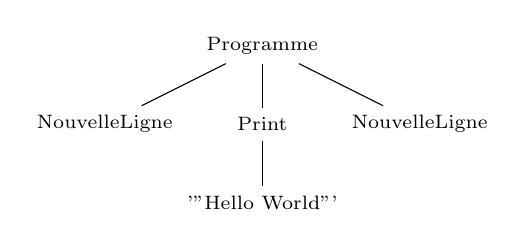
\begin{tikzpicture}
    \node[font=\scriptsize] (0) at (0, 0) {Programme};
    \node[font=\scriptsize] (1) at (-2, -1) {NouvelleLigne};
    \node[font=\scriptsize] (2) at (0, -1) {Print};
    \node[font=\scriptsize] (3) at (0, -2) {'"Hello World"'};
    \node[font=\scriptsize] (4) at (2, -1) {NouvelleLigne};
    
    \draw (0) -- (1);
    \draw (0) -- (2);
    \draw (2) -- (3);
    \draw (0) -- (4);
\end{tikzpicture}}
      };

      \draw [lien, thick] (Fortran.south) to (C.north);
    \end{scope}
  \end{tikzpicture}
\end{frame}

\newcommand{\drawcross}[1]{
  \draw[cross] (#1.north west) -- (#1.south east);
  \draw[cross] (#1.north east) -- (#1.south west);
}

\tikzstyle{cross}=[red, very thick]

%--------------expilaction---------------
\subsection{Fonctionnement}
\begin{frame}
  \frametitle{Syntaxe abstraite\esp}

  \begin{tikzpicture}
    % frame
    \node[frame] (frame) {};
    \tikzstyle{faded}=[draw=black!20,color=black!20]
    
    \node[below=4cm of frame.west, anchor=west, box, faded] (state_1) {\scriptsize Analyse lexicale};
    \node[right=0.5cm of state_1.east, anchor=west, box, faded] (state_2) {\scriptsize Analyse syntaxique};
    \node[right=0.5cm of state_2.east, anchor=west, box] (state_3) {\scriptsize Abstraction};
    \node[right=0.5cm of state_3.east, anchor=west, box, faded] (state_4) {\scriptsize Conversion};
    \draw[->, >=latex, faded] (state_1.east) -- (state_2.west);
    \draw[->, >=latex, faded] (state_2.east) -- (state_3.west);
    \draw[->, >=latex, faded] (state_3.east) -- (state_4.west);
    \draw[dashed] (frame.south west) -- (state_3.north west);
    \draw[dashed] (frame.south east) -- (state_3.north east);

    % definition
    \begin{scope}[shift={(-3, 2)}, font=\footnotesize]
      \node (0) at (0, 0) {S};
      \node [below=0.3cm of 0] (1) {A};
      \node [below=0.3cm of 1.south west] (2) {a};
      \node [below=0.3cm of 1.south east] (3) {A};
      \node [below=0.3cm of 3] (4) {B};
      \node [below=0.3cm of 4.south west] (5) {b};
      \node [below=0.3cm of 4.south east] (6) {B};
      \node [below=0.3cm of 6] (7) {$\varepsilon$};

      \draw (0) -- (1);
      \draw (1) -- (2);
      \draw (1) -- (3);
      \draw (3) -- (4);
      \draw (4) -- (5);
      \draw (4) -- (6);
      \draw (6) -- (7);
    
      
      \only<2->{\drawcross{3}}
      \only<3->{\drawcross{6}}
      \only<4->{\drawcross{7}}
      
      \only<5->{
        \node[right=0.8cm of 3, font=\ttfamily] {$\Rightarrow$};

        \node [right=2.5cm of 0] (_0) {S};
        \node [below=0.3cm of _0] (_1) {A};
        \node [below=0.3cm of _1.south west] (_2) {a};
        \node [below=0.3cm of _1.south east] (_4) {B};
        \node [below=0.3cm of _4.south] (_5) {b};

        \draw (_0) -- (_1);
        \draw (_1) -- (_2);
        \draw (_1) -- (_4);
        \draw (_4) -- (_5);
      }

      \only<6->{\draw[->, >=latex, draw=blue, very thick] (_4) [bend right] to (_0);}

      \only<7>{
        \node[right=0.8cm of _4, font=\ttfamily] {$\Rightarrow$};

        \node [right=2.5cm of _1] (__0) {S};
        \node [below=0.3cm of __0.south west] (__1) {A};
        \node [below=0.3cm of __1.south] (__2) {a};
        \node [below=0.3cm of __0.south east] (__4) {B};
        \node [below=0.3cm of __4.south] (__5) {b};

        \draw (__0) -- (__1);
        \draw (__1) -- (__2);
        \draw (__0) -- (__4);
        \draw (__4) -- (__5);
        }
    \end{scope}

  \end{tikzpicture}

\end{frame}

%----------un exemple----------
\subsection{Un exemple}
\begin{frame}
  \scalebox{0.8}{\tikzstyle{feuille}=[]
\tikzstyle{noeud}=[]
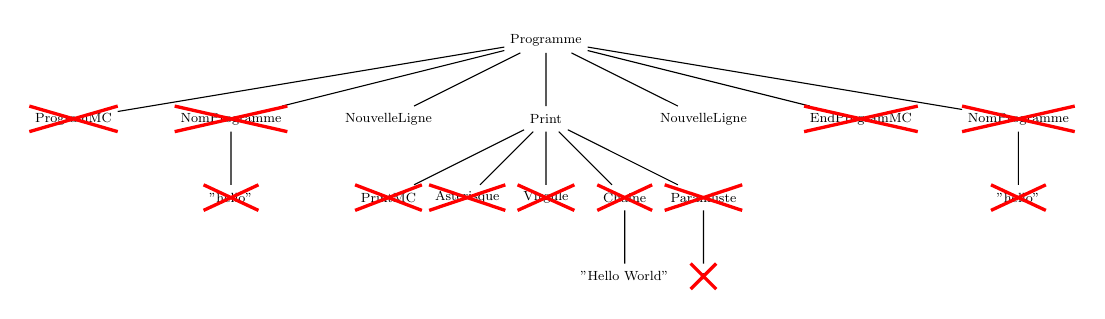
\begin{tikzpicture}
    [
        baseline=(0), 
        level/.style={sibling distance = 2cm/#1, level distance = 1cm},
        every node/.style={scale=0.6, font=\footnotesize, minimum width=15pt, minimum height=15pt}
    ]
    
    \node at (0, 0) { };
    \begin{scope}[shift={(5, 0)}]
        \node {Programme}
            child {node (0) {ProgramMC}}
            child {node (1) {NomProgramme}
                child {node (2) {"hello"}}
            }
            child {node {NouvelleLigne}}
            child {node {Print}
                child {node (3) {PrintMC}}
                child {node (4) {Asterisque}}
                child {node (5) {Virgule}}
                child {node (6) {Chaine}
                    child {node {"Hello World"}}
                }
                child{node (7) {Paramliste}
                    child {node (8) {$\varepsilon$}}
                }
            }
            child {node {NouvelleLigne}}
            child {node (9) {EndProgramMC}}
            child {node (10) {NomProgramme}
                child {node (11) {"hello"}}
            }
        ;
        \only<2>{\foreach \step in {0,1,...,11}{\drawcross{\step}}}
    \end{scope}
\end{tikzpicture}}
\end{frame}

\begin{frame}
  \begin{center}
    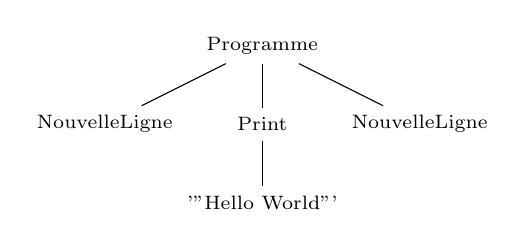
\begin{tikzpicture}
    \node[font=\scriptsize] (0) at (0, 0) {Programme};
    \node[font=\scriptsize] (1) at (-2, -1) {NouvelleLigne};
    \node[font=\scriptsize] (2) at (0, -1) {Print};
    \node[font=\scriptsize] (3) at (0, -2) {'"Hello World"'};
    \node[font=\scriptsize] (4) at (2, -1) {NouvelleLigne};
    
    \draw (0) -- (1);
    \draw (0) -- (2);
    \draw (2) -- (3);
    \draw (0) -- (4);
\end{tikzpicture}
  \end{center}
\end{frame}